% arara: xelatex: {synctex: true}
% arara: indent: {overwrite: yes}
\documentclass[]{IMTexam}

\usepackage[enums]{IMTtikz}

\givecredits
\author{Isabella B.}
\USPN{11810773}
\date{}
\lecture{Física I} % disciplina
\lcode{4302111}
\hwtype{Resolução} % o que é
\examname{Provinha X} % prova

\begin{document}

\maketitle

\begin{questions}

	\question\label{ques:q1} Vamos estudar o problema de 2 corpos que interagem por meio de uma força central, $ \vec{F} \parallel \vec{r} $, onde $ \vec{r} $ é o vetor posição relativa entre os corpos. Para começar, vamos utilizar os vetores $ \vec{r_1} $ e $ \vec{r_2} $, que são os vetores posição das partículas em um certo referencial. Suponha que os corpos tenham massas $ m_1 $ e $ m_2 $, respectivamente. Nosso objetivo aqui será mostrar que este problema pode ser transformado em um problema efetivo, possuindo apenas uma partícula com massa igual à massa reduzida.

	\begin{parts}
		\part \label{part:q1a} Escreva a segunda lei de Newton para cada um dos corpos, supondo inicialmente que eles interagem por meio da lei universal da gravitação de Newton.

		\begin{solution}
			Sendo a força de interação entre os dois corpos $ \vec{F} $, temos, pela segunda lei de Newton, as seguintes equações de movimento:
			\begin{gather}
				-\vec{F}=m_1\,\vec{\ddot{r}_1}\label{eq:Fm1}\\
				\vec{F}=m_2\,\vec{\ddot{r}_2}\label{eq:Fm2}
			\end{gather}

			\paragraph{Nota:} $\vec{F}$ é negativa para o corpo 1 pois é a reação da força (terceira lei de Newton).
		\end{solution}

		Considere as seguintes variáveis
		\begin{gather}
			\vec{r} = \vec{r_2} - \vec{r_1},\label{eq:eq1}\\
			\vec{R}=\dfrac{m_1\,\vec{r_1}+m_2\,\vec{r_2}}{m_1+m_2}.\label{eq:eq2}
		\end{gather}

		\part \label{part:q1b} Inverta as relações acima para escrever $ \vec{r_1} $, $ \vec{r_2} $ em termos de $ \vec{r}, \vec{R} $.

		\begin{solution}
			A partir de \ref{eq:eq2}, temos
			\begin{align}
				\vec{R}   & =\dfrac{m_2\del{\vec{r_2}-\vec{r_1}}+\del{m_1+m_2}\vec{r_1}}{m_1+m_2}\nonumber  \\
				\intertext{substituindo \ref{eq:eq1}}
				          & =\dfrac{m_2\,\vec{r}+\del{m_1+m_2}\vec{r_1}}{m_1+m_2}\nonumber                  \\
				\intertext{isolando $ \vec{r_1} $, ficamos com}
				\vec{r_1} & =\vec{R}-\dfrac{m_2}{\del{m_1+m_2}}\,\vec{r}\label{eq:r1Rr}                     \\
				\intertext{por processo análogo, temos}
				\vec{R}   & =\dfrac{-m_1\del{\vec{r_2}-\vec{r_1}}+\del{m_1+m_2}\vec{r_2}}{m_1+m_2}\nonumber \\
				\vec{r_2} & =\vec{R}+\dfrac{m_1}{\del{m_1+m_2}}\,\vec{r}\label{eq:r2Rr}
			\end{align}
		\end{solution}

		\part \label{part:q1c} Agora, utilizando os resultados do item anterior e as equações \ref{eq:eq1} e \ref{eq:eq2}, mostre que as equações de Newton para $ \vec{r_1} $ e $ \vec{r_2} $ podem ser escritas como%
		\footnote{Dica: Some e subtraia as equações. O resultado \ref{eq:eq3} é obtido diretamente. Já para a equação \ref{eq:eq4} será necessário utilizar as relações inversas obtidas no item \ref{part:q1b}.}
		\begin{gather}
			\ddot{\vec{R}}=\vec{0},\label{eq:eq3}\\
			\mu\,\ddot{\vec{r}}=-G\dfrac{m_1\,m_2}{r^{3}}\,\vec{r},\label{eq:eq4}
		\end{gather}
		onde $ \mu  = m_1\,m_2/(m_1 + m_2) $ é a massa reduzida. Isto nos mostra que as variáveis $ \set{\vec{r},\vec{R}} $ são ideais para estudar o problema de dois corpos!

		\begin{solution}
			Tomando a segunda derivada de \ref{eq:eq2}, temos
			\begin{align*}
				\vec{\ddot{R}} & =\dfrac{m_1\,\vec{\ddot{r}_1}+m_2\,\vec{\ddot{r}_2}}{m_1+m_2}              \\
				\intertext{substituindo \ref{eq:Fm1} e \ref{eq:Fm2}}
				\vec{\ddot{R}} & =\dfrac{-m_1\dfrac{\vec{F}}{m_1}+m_2\dfrac{\vec{F}}{m_2}}{m_1+m_2}=\vec{0}
			\end{align*}

			%			Reescrevendo \ref{eq:r1Rr} e \ref{eq:r2Rr} através da massa reduzida, temos
			%			\begin{gather}
			%				\vec{r_1}=\vec{R}-\dfrac{\mu}{m_1}\vec{r}\\
			%				\vec{r_2}=\vec{R}+\dfrac{\mu}{m_2}\vec{r}
			%			\end{gather}
			Tomando a segunda derivada de \ref{eq:eq1}, temos
			\begin{align*}
				\vec{\ddot{r}}      & = \vec{\ddot{r}_2}-\vec{\ddot{r}_1}          \\
				\intertext{substituindo \ref{eq:Fm1} e \ref{eq:Fm2}}
				\vec{\ddot{r}}      & = \dfrac{\vec{F}}{m_2}+ \dfrac{\vec{F}}{m_1} \\
				\vec{\ddot{r}}      & = \dfrac{\vec{F}\del{m_1+m_2}}{m_1\,m_2}     \\
				\mu\vec{\ddot{r}}   & =\vec{F}                                     \\
				\intertext{sendo $ \vec{F} $ uma força central (portanto, atua na direção radial $ \rhat=\vec{r}/r $, para $ r=|\vec{r}| $) e é diretamente proporcional às massas dos corpos envolvidos, inversamente proporcional ao quadrado da distância entre eles e atrativa, podemos escrever:}
				\mu\,\vec{\ddot{r}} & =-G\dfrac{m_1\,m_2}{r^{3}}\,\vec{r}.
			\end{align*}

			\hfill\qedsymbol
		\end{solution}

		Embora tenhamos começado supondo a lei da gravitação de Newton, estas variáveis são ótimas para qualquer problema de força central%
		\footnote{Vocês vão utilizar estas coordenadas tanto em Relatividade Geral, como será visto abaixo, como para resolver o átomo de Hidrogênio em mecânica quântica.}.

		Isso se deve ao fato de que para o potencial a única informação relevante é a distância relativa entre as partículas. Deste modo, embora estando estudando a dinâmica de duas partículas, podemos nos preocupar apenas com uma equação:
		\begin{equation}\label{eq:eq5}
			\mu\,\ddot{\vec{r}}=\vec{F}=-\dpd{V(r)}{r}\rhat
		\end{equation}

		Ainda existem outras propriedades do problema de dois corpos que podemos utilizar para resolver a equação \ref{eq:eq5}. São elas a conservação de energia e do momento angular.


	\end{parts}

	\question\label{ques:q2}

	\begin{parts}
		\part \label{part:q2a} Utilizando o vetor aceleração em coordenadas polares obtenha as componentes radial e angular da equação \ref{eq:eq5}.

		\begin{solution}
			Sendo o vetor posição em coordenadas polares
			\begin{equation}\label{eq:rrhat}
				\vec{r}=r\,\rhat,
			\end{equation}
			e as derivadas dos versores $ \rhat $ e $ \that $ respectivamente
			\begin{gather}
				\dot{\rhat}=\dot{\theta}\,\that\label{eq:drhat},\\
				\dot{\that}=-\dot{\theta}\,\rhat\label{eq:dthat}.
			\end{gather}

			Tomando a segunda derivada de \ref{eq:rrhat}, temos
			\begin{align*}
				\vec{\ddot{r}} & =\dod{}{t}\sbr{\dot{r}\,\rhat+r\,\dot{\rhat}}                                                                            \\
				               & =\dod{}{t}\sbr{\dot{r}\,\rhat+r\,\dot{\theta}\,\that}                                                                    \\
				               & =\ddot{r}\,\rhat+\dot{r}\,\dot{\rhat}+\dot{r}\,\dot{\theta}\,\that+r\del{\ddot{\theta}\,\that+\dot{\theta}\,\dot{\that}} \\
				               & =\ddot{r}\,\rhat+2\dot{r}\,\dot{\theta}\,\that+r\,\ddot{\theta}\,\that-r\,\dot{\theta}^{2}\,\rhat                        \\
				\vec{\ddot{r}} & =\del{\ddot{r}-r\,\dot{\theta}^{2}}\rhat+\del{2\dot{r}\,\dot{\theta}+r\,\ddot{\theta}}\that
			\end{align*}

			Pela equação \ref{eq:eq5}, temos
			\begin{gather}
				\ddot{r}-r\,\dot{\theta}^{2}=-\dfrac{1}{\mu}\dpd{V(r)}{r}\label{eq:radcomp}\\
				2\dot{r}\,\dot{\theta}+r\,\ddot{\theta}=0\label{eq:angcomp}
			\end{gather}

		\end{solution}

		\part \label{part:q2b} Analise a equação na componente $ \that $ e mostre que ela pode ser integrada diretamente, fornecendo uma constante de integração $ l\equiv \mu\,r^{2}\,\dot{\theta} $, que é o momento angular efetivo.

		\begin{solution}
			Multiplicando \ref{eq:angcomp} por $ \mu\,r $, temos
			\begin{align}
				\mu\del{2r\,\dot{r}\,\dot{\theta}+r^{2}\,\ddot{\theta}}                      & =0\nonumber                                                                                                                             \\
				\intertext{integrando com respeito ao tempo:}
				\mu\int\sbr{2r\,\dot{r}\,\dot{\theta}+r^{2}\,\ddot{\theta}}\dif t            & =\int 0\dif t\nonumber                                                                                                                  \\
				\mu\int 2r\,\dot{r}\,\dot{\theta} \dif t+\mu \int r^{2}\,\ddot{\theta}\dif t & =C\nonumber                                                                                                                             \\
				\intertext{do lado direito $ C=l= $ const. e, do lado esquerdo, aplicamos a regra de integração por partes, com $ \dif f=\ddot{\theta}\dif t\implies f=\dot{\theta} $}
				l                                                                            & =\cancel{\mu\int 2r\,\dot{r}\,\dot{\theta} \dif t}+\mu \del{r^{2}\,\dot{\theta}-\cancel{\int 2r\,\dot{r}\,\dot{\theta}\dif t}}\nonumber \\
				l                                                                            & =\mu\,r^{2}\,\dot{\theta}\label{eq:lmrtdot}
			\end{align}

			\hfill\qedsymbol
		\end{solution}

		\part \label{part:q2c} Analise a equação na direção $ \vec{r} $ e mostre que ela pode ser escrita como
		\begin{equation}\label{eq:eq6}
			\dod{E}{t}=0.
		\end{equation}

		Dicas:
		\begin{enumerate}
			\item Comece eliminando $ \dot{\theta} $ em termos do momento angular, dado por
			      \begin{equation}\label{eq:eq7}
				      \dot{\theta}=\dfrac{l}{\mu\,r^{2}}\,;
			      \end{equation}

			\item Multiplique os dois lados da igualdade por $ \dot{r} $ e utilize a regra da cadeia para simplificar a expressão, e transformá-la em algo da forma
			      \begin{equation}\label{eq:eq8}
				      \dod{f}{t}=0\,;
			      \end{equation}

			\item Finalmente identifique que o termo sendo derivado tem dimensão de energia e é justamente a energia total do sistema.

			      É útil perceber que $ \dot{r}\,\ddot{r}=\od{(\dot{r}^{2}/2)}{t} $.

		\end{enumerate}

		\begin{solution}
			Tomando \ref{eq:radcomp}, temos
			\begin{align}
				\ddot{r}-r\,\dot{\theta}^{2}                                                                & =-\dfrac{1}{\mu}\dpd{V(r)}{r} \\
				\intertext{substituindo $ \dot{\theta}=l/(\mu\,\r^{2}) $ (de \ref{eq:lmrtdot})}
				\ddot{r}-r\del{\dfrac{l}{\mu\,r^{2}}}^{2}                                                   & =-\dfrac{1}{\mu}\dpd{V(r)}{r} \\
				\mu\,\ddot{r}\,\dot{r}-\dfrac{l^{2}\,\dot{r}}{\mu\,r^{3}}                                   & =-\dot{r}\,\dpd{V(r)}{r}      \\
				\mu\,\dod{(\dot{r}^{2}/2)}{t}+\dod{}{t}\sbr{-\dfrac{l^{2}}{\mu}\int \dfrac{1}{r^{3}}\dif r} & =-\dod{}{t}\sbr{V(r)}         \\
				\dod{}{t}\sbr{V(r)+\dfrac{l^{2}}{\mu}\dfrac{1}{2r^{2}}+\dfrac{\mu\,\dot{r}^{2}}{2}}         & =0\label{eq:Vrbig}
			\end{align}
			Analisando as dimensões de cada termo em \ref{eq:Vrbig}, temos
			\begin{gather*}
				\sbr{V(r)}=M\del{\dfrac{L}{T}}^{2}\quad\text{já que se trata de um potencial}\\
				\sbr{\dfrac{l^{2}}{2\mu\,r^{2}}}=\sbr{\dfrac{\del{\mu\,r^{2}\,\dot{\theta}}^{2}}{\mu\,r^{2}}}=\sbr{\mu\,r^{2}\dot{\theta}^{2}}=M\del{\dfrac{L}{T}}^{2}\\
				\sbr{\dfrac{\mu\,\dot{r}^{2}}{2}}=M\del{\dfrac{L}{T}}^{2}
			\end{gather*}
			Portanto, estamos derivando um termo de energia.
		\end{solution}

		De volta à equação de Newton na direção $ \rhat $, ela pode ser escrita como a equação do movimento para uma partícula sujeita a um potencial efetivo
		\begin{equation}\label{eq:eq9}
			V_{\textup{efetivo}}=V(r)+\dfrac{l^{2}}{2\mu\,r^{2}}
		\end{equation}

		Este último termo do potencial efetivo é chamado de barreira centrifuga e é bastante peculiar%
		\footnote{Enfatizamos que os resultados obtidos valem para qualquer problema de força central. Isso nos da a liberdade de estudar diferentes teorias, bastando utilizar o potencial central $ V(r) $ associado.}.

		\part \label{part:q2d} Mostre que a força gerada pela barreira centrifuga é de repulsão e é tão grande quanto menor for a distancia relativa entre as partículas.

		\begin{solution}
			Sendo o último termo de \ref{eq:eq9} um potencial, temos que a força dada por ele será igual ao oposto de sua derivada com respeito à distância. Dessa forma
			\begin{align*}
				F & =-\dpd{}{r}\sbr{\dfrac{l^{2}}{2\mu\,r^{2}}} \\
				F & =\dfrac{l^{2}}{\mu\,r^{3}}.
			\end{align*}
			Como o módulo da força é positivo, sabemos que ela é de repulsão e, além disso, ela é inversamente proporcional ao cubo da distância.

			\hfill\qedsymbol
		\end{solution}

		\part \label{part:q2e} Suponha que a força entre as partículas seja gravitacional. Faça um gráfico mostrando o comportamento deste potencial em função de $ r $. Sugiro utilizar a constante de Newton valendo 1 para melhorar a visualização dos efeitos. Sugiro também fazer várias curvas no mesmo gráfico:

		\begin{enumerate}
			\item Algumas fixando $ \mu=1 $ e variando $ l=\numlist{0.1;0.5} $;
			\item Algumas fixando $ l = 1 $ e variando $ \mu = \numlist{0.1;0.5;1} $ para observar como se modificam essa curvas.
		\end{enumerate}

		Discuta a mudança no formato dessas curvas e o significado físico destes efeitos.

		\begin{solution}
			Sabemos que o potencial gravitacional é dado pelo oposto da integral da força na distância do infinito à $ r $. Dessa forma:
			\begin{equation}\label{eq:Vpot}
				V(r)=-\int_\infty^r \vec{F}\cdot\dif\vec{r}=-\int_\infty^r -G\dfrac{m_1\,m_2}{r^{'3}}\,\vec{r}\cdot\del{\rhat\dif r'+r'\,\that\dif \theta}=-\int_\infty^r G\dfrac{m_1\,m_2}{r^{'2}}\dif r'=-G\dfrac{m_1\,m_2}{r}
			\end{equation}

			Fazendo $ m_1\,m_2=1 $ e $ G=1 $ temos
			\begin{center}
				\begin{minipage}{0.8\linewidth}
					\centering
					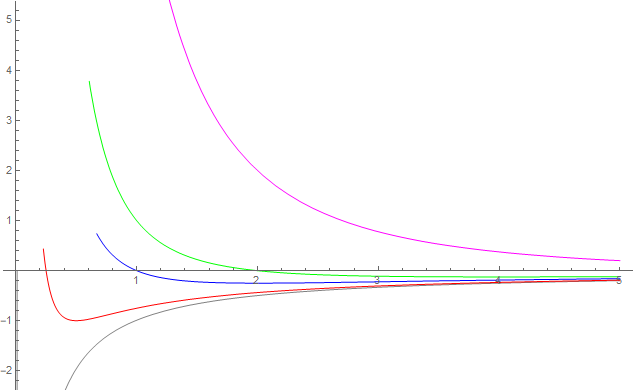
\includegraphics[width=1\linewidth]{Graph1}
				\end{minipage}\hfill
				\begin{minipage}{0.15\linewidth}
					\centering
					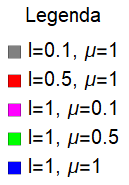
\includegraphics[width=1\linewidth]{leg1}
				\end{minipage}
			\end{center}

		\end{solution}

		\part \label{part:q2f} Agora suponha que que as duas esferas tenham carga elétrica $ +Q $, e que o potencial $ V(r) $ seja o potencial de Coulomb. Faça um gráfico mostrando o comportamento do potencial neste caso também (para plotar, você pode supor este potencial como sendo $ V(r) = k/r $, onde $ k $ é uma constante positiva. Escolha diferentes valores para esta constante de modo a deixar claro seu efeito no potencial efetivo).

		\begin{solution}
			Fazendo $ l=1 $, e um equivalente da massa reduzida $ \mu_e $ (carga reduzida?), temos

			\begin{center}
				\begin{minipage}{0.8\linewidth}
					\centering
					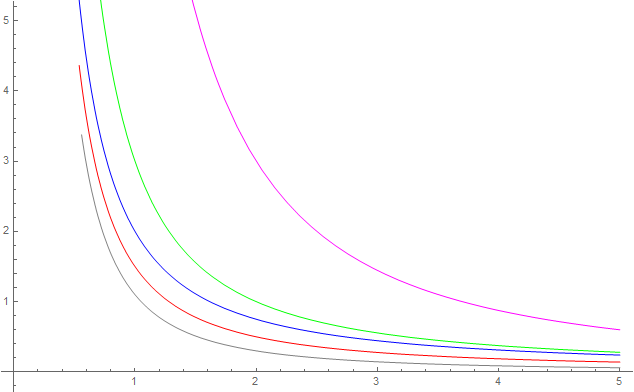
\includegraphics[width=1\linewidth]{Graph2}
				\end{minipage}\hfill
				\begin{minipage}{0.15\linewidth}
					\centering
					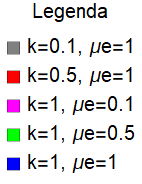
\includegraphics[width=1\linewidth]{leg2}
				\end{minipage}
			\end{center}
		\end{solution}

	\end{parts}

	\extra{Problema Extra}

	Na teoria da relatividade de Einstein, será possível transformar um problema de dois corpos atraídos pela força da gravidade em um problema unidimensional, envolvendo um só corpo, da mesma forma que fizemos acima. Neste caso, no entanto, o potencial efetivo será um pouco diferente%
	\footnote{Na equação \ref{eq:eq10} estamos usando que a velocidade da luz é dada por $ c = 1 $, sendo adimensional.},
	\begin{equation}\label{eq:eq10}
		V_{\textup{efetivo}}(r)=-\dfrac{G\,m_1\,m_2}{r}+\dfrac{l^{2}}{2\mu\,r^{2}}-\dfrac{G\del{m_1+m_2}l^{2}}{\mu\,r^{3}}
	\end{equation}
	note que os termos $ -G\mu^{2}/r $ e $ l^{2}/2\mu\,r^{2} $ já estavam presentes na teoria Newtoniana. A grande diferença está no último termo. Faça um gráfico mostrando o comportamento deste potencial efetivo como função de $ r $.

	Você deve perceber uma grande diferença. No caso Newtoniano para raios pequenos, víamos o potencial crescer indefinidamente: este comportamento é chamado de \textbf{barreira centrífuga}, e surge pois é muito difícil orbitar uma massa pontual em raios muito pequenos, visto que a força centrípeta teria que ser enorme. Já no caso da Relatividade Geral, vemos que em $ r = 2G\,\mu $  todas as curvas do potencial se cruzam, e que para raios menores ele passa a se tornar cada vez mais negativo, divergindo em direção a $ -\infty $. Isso ocorre, pois a partir desse raio se encontra a região chamada \textbf{buraco negro}, da qual não é possível escapar: qualquer partícula que vá para $ r<2G\,\mu $ será forçada a descer esse poço de potencial, eventualmente chegando a $ r = 0 $.

	Dica: Para conseguir fazer este gráfico, é conveniente utilizar $ G\,m_1=1 $, e também utilizar a coordenada radial $ r'=r/2G\,\mu $.

	\begin{solution}
		\begin{align*}
			V_{\textup{efetivo}}(r)  & =-\dfrac{G\,m_1\,m_2}{r}+\dfrac{l^{2}}{2\mu\,r^{2}}-\dfrac{G\del{m_1+m_2}l^{2}}{\mu\,r^{3}}                                                                     \\
			                         & =r^{-3}\del{-G\,m_1\,m_2\,r^{2}+\dfrac{l^{2}\,r}{2\mu}-\dfrac{G\del{m_1+m_2}l^{2}}{\mu}}                                                                        \\
			\intertext{substituindo $ r=r'\,2G\,\mu $}
			                         & =\del{r'\,2G\,\mu}^{-3}\del{-G\,m_1\,m_2\del{r'\,2G\,\mu}^{2}+\dfrac{l^{2}\del{r'\,2G\,\mu}}{2\mu}-\dfrac{G\del{m_1+m_2}l^{2}}{\mu}}                            \\
			\intertext{adotando $ m_1=m_2=m\implies \mu=m/2 $ e $ G=1 $, temos}
			                         & =\del{r'\,2\cdot1\dfrac{m}{2}}^{-3}\del{-1m^{2}\del{r'\,2\cdot1\dfrac{m}{2}}^{2}+\dfrac{l^{2}\del{r'\,2\cdot1\dfrac{m}{2}}}{2m/2}-\dfrac{1\cdot2m\,l^{2}}{m/2}} \\
			V_{\textup{efetivo}}(r') & =-\dfrac{m}{r'}+\dfrac{l^{2}}{m^{3}\,r^{\prime2}}-\dfrac{4l^{2}}{m^{3}\,r^{\prime3}}
		\end{align*}
	\end{solution}

\end{questions}
\end{document}
